\documentclass[final, 3p, times, 11.5pt]{article}

\usepackage[english]{babel}
\usepackage[utf8]{inputenc}
\usepackage[T1]{fontenc}

% Dokumentformatering:
\setlength\parindent{0pt} %ingen innrykk
\usepackage[parfill]{parskip} % Mellomrom mellom avsnitt
% Endre str
\usepackage[a4paper,top=3cm,bottom=2cm,left=1.5cm,right=1.5cm,marginparwidth=1.75cm]{geometry} % utnytter større del av arket.
\usepackage{appendix}
\usepackage{multicol}
\usepackage{titlesec}
\titleformat{\chapter}[display]
  {\normalfont\huge\bfseries}{\chaptertitlename\ \thechapter}{20pt}{\Huge}
\titlespacing*{\chapter}{0pt}{-70pt}{20pt} % reduce headspace of the chapter title
\setcounter{secnumdepth}{0} % Set the depth of section numbering to subsubsections



% Matte og symboler
\usepackage{lmodern}
\usepackage{textcomp, gensymb}
\usepackage{amssymb}
\usepackage{amsmath}
\usepackage{mathtools}
\usepackage{physics}
\usepackage{cancel} % Gjennomstreking i likninger etc
\usepackage{amsthm}
\usepackage{caption}
\usepackage{dirtytalk}
\usepackage{cancel}

% Pseudocode
\usepackage{algorithm}
\usepackage{algpseudocode}

% Håndterer grafikk:
\usepackage{graphicx}
\graphicspath{{Figures/}} % Henter grafikk fra mappen "Figurer"
\usepackage{wrapfig}
\setlength{\intextsep}{2pt} % adjust vertical space above and below the wrapfigure
\usepackage{subcaption} % eller subfigure
\usepackage[font=small,labelfont=bf]{caption} % Mindre figurtekst, bold på figur numerering
\usepackage{transparent} % Kan gjøre tekst mere gjenomsiktig
\usepackage{listings}
\usepackage{paralist}
\usepackage{tikz}
\usetikzlibrary{matrix}
\usetikzlibrary{fit}
\usetikzlibrary{intersections}
\usepackage{multirow}
\usepackage{pdfpages} % sett in pdf i dokumentet
\usepackage{subcaption} 
\usepackage{tabularx}
\usepackage{tabularray} % beste tabellpakke
\usepackage{pgfplots}
\usepgfplotslibrary{fillbetween}
\pgfplotsset{width=10cm,compat=1.9}
\newcommand{\tabitem}{~~\llap{\textbullet}~~} % for kulepunkter i tabeller uten vspace over dem

% Håndterer fine tabeller:
\usepackage{booktabs}
\usepackage{multirow}

% Håntere kilder med hyperlinker
\usepackage{csquotes}
\usepackage{hyperref}
\hypersetup{
    colorlinks=true,        % Colored links instead of frames
    linkcolor=blue,         % Color for internal links
    citecolor=red,          % Color for citations
    urlcolor=red            % Color for external links
}
\usepackage[style=numeric, sorting=none]{biblatex} 
\addbibresource{sources.bib}
\usepackage{lastpage} 
\usepackage[printonlyused,withpage]{acronym}
\usepackage{footmisc}




% Egne funksjoner
\newcommand{\frontmatter}{\cleardoublepage \pagenumbering{roman}}
\newcommand{\mainmatter}{\cleardoublepage \pagenumbering{arabic}}

\usepackage{caption}
\captionsetup{%
    ,format=hang
    ,justification=raggedright
    ,singlelinecheck=false
    ,figureposition=top
    }


\makeatletter
\AtBeginDocument{%
  \renewcommand*{\AC@hyperlink}[2]{%
    \begingroup
      \hypersetup{hidelinks}%
      \hyperlink{#1}{#2}%
    \endgroup
  }%
}
\makeatother





% Håndterer multi-fil oppsett:
\usepackage{xr}
\usepackage{subfiles}
\externaldocument{\subfix{main}}
 
\graphicspath{{Project 2/Figures/}}

\begin{document}
\section{Problem 1}

Let the equation 
\begin{equation}\label{eq:1d_buckling_beam}
        \gamma \frac{d^2 u(x)}{dx^2} = - F u(x) \quad ,
\end{equation}

where $\gamma$ is some constant defined by material properties like rigidity, describe a case where we have a horizontal beam where:
    \begin{itemize}
        \item $L$ is the horizontal length between the two beam endpoints. (So before any buckling, $L$ is also the length of the beam.)
        \item We let $u(x)$ be the vertical displacement of the beam at horizontal position $x$, with $x \in [0,L]$.
        \item A force $F$ is applied at the endpoint ($x=L$), *directed into the beam*, i.e. towards $x=0$. 
        \item The beam is fastened with \textit{pin endpoints}, meaning that $u(0)=0$ and $u(L)=0$, but the endpoints are allowed to rotate ($u'(x) \neq 0$).
    \end{itemize}

An illustration with the key definitions are provided in Figure \ref{fig:beam_illustration}. 

\begin{figure}[h!]
    \centering
    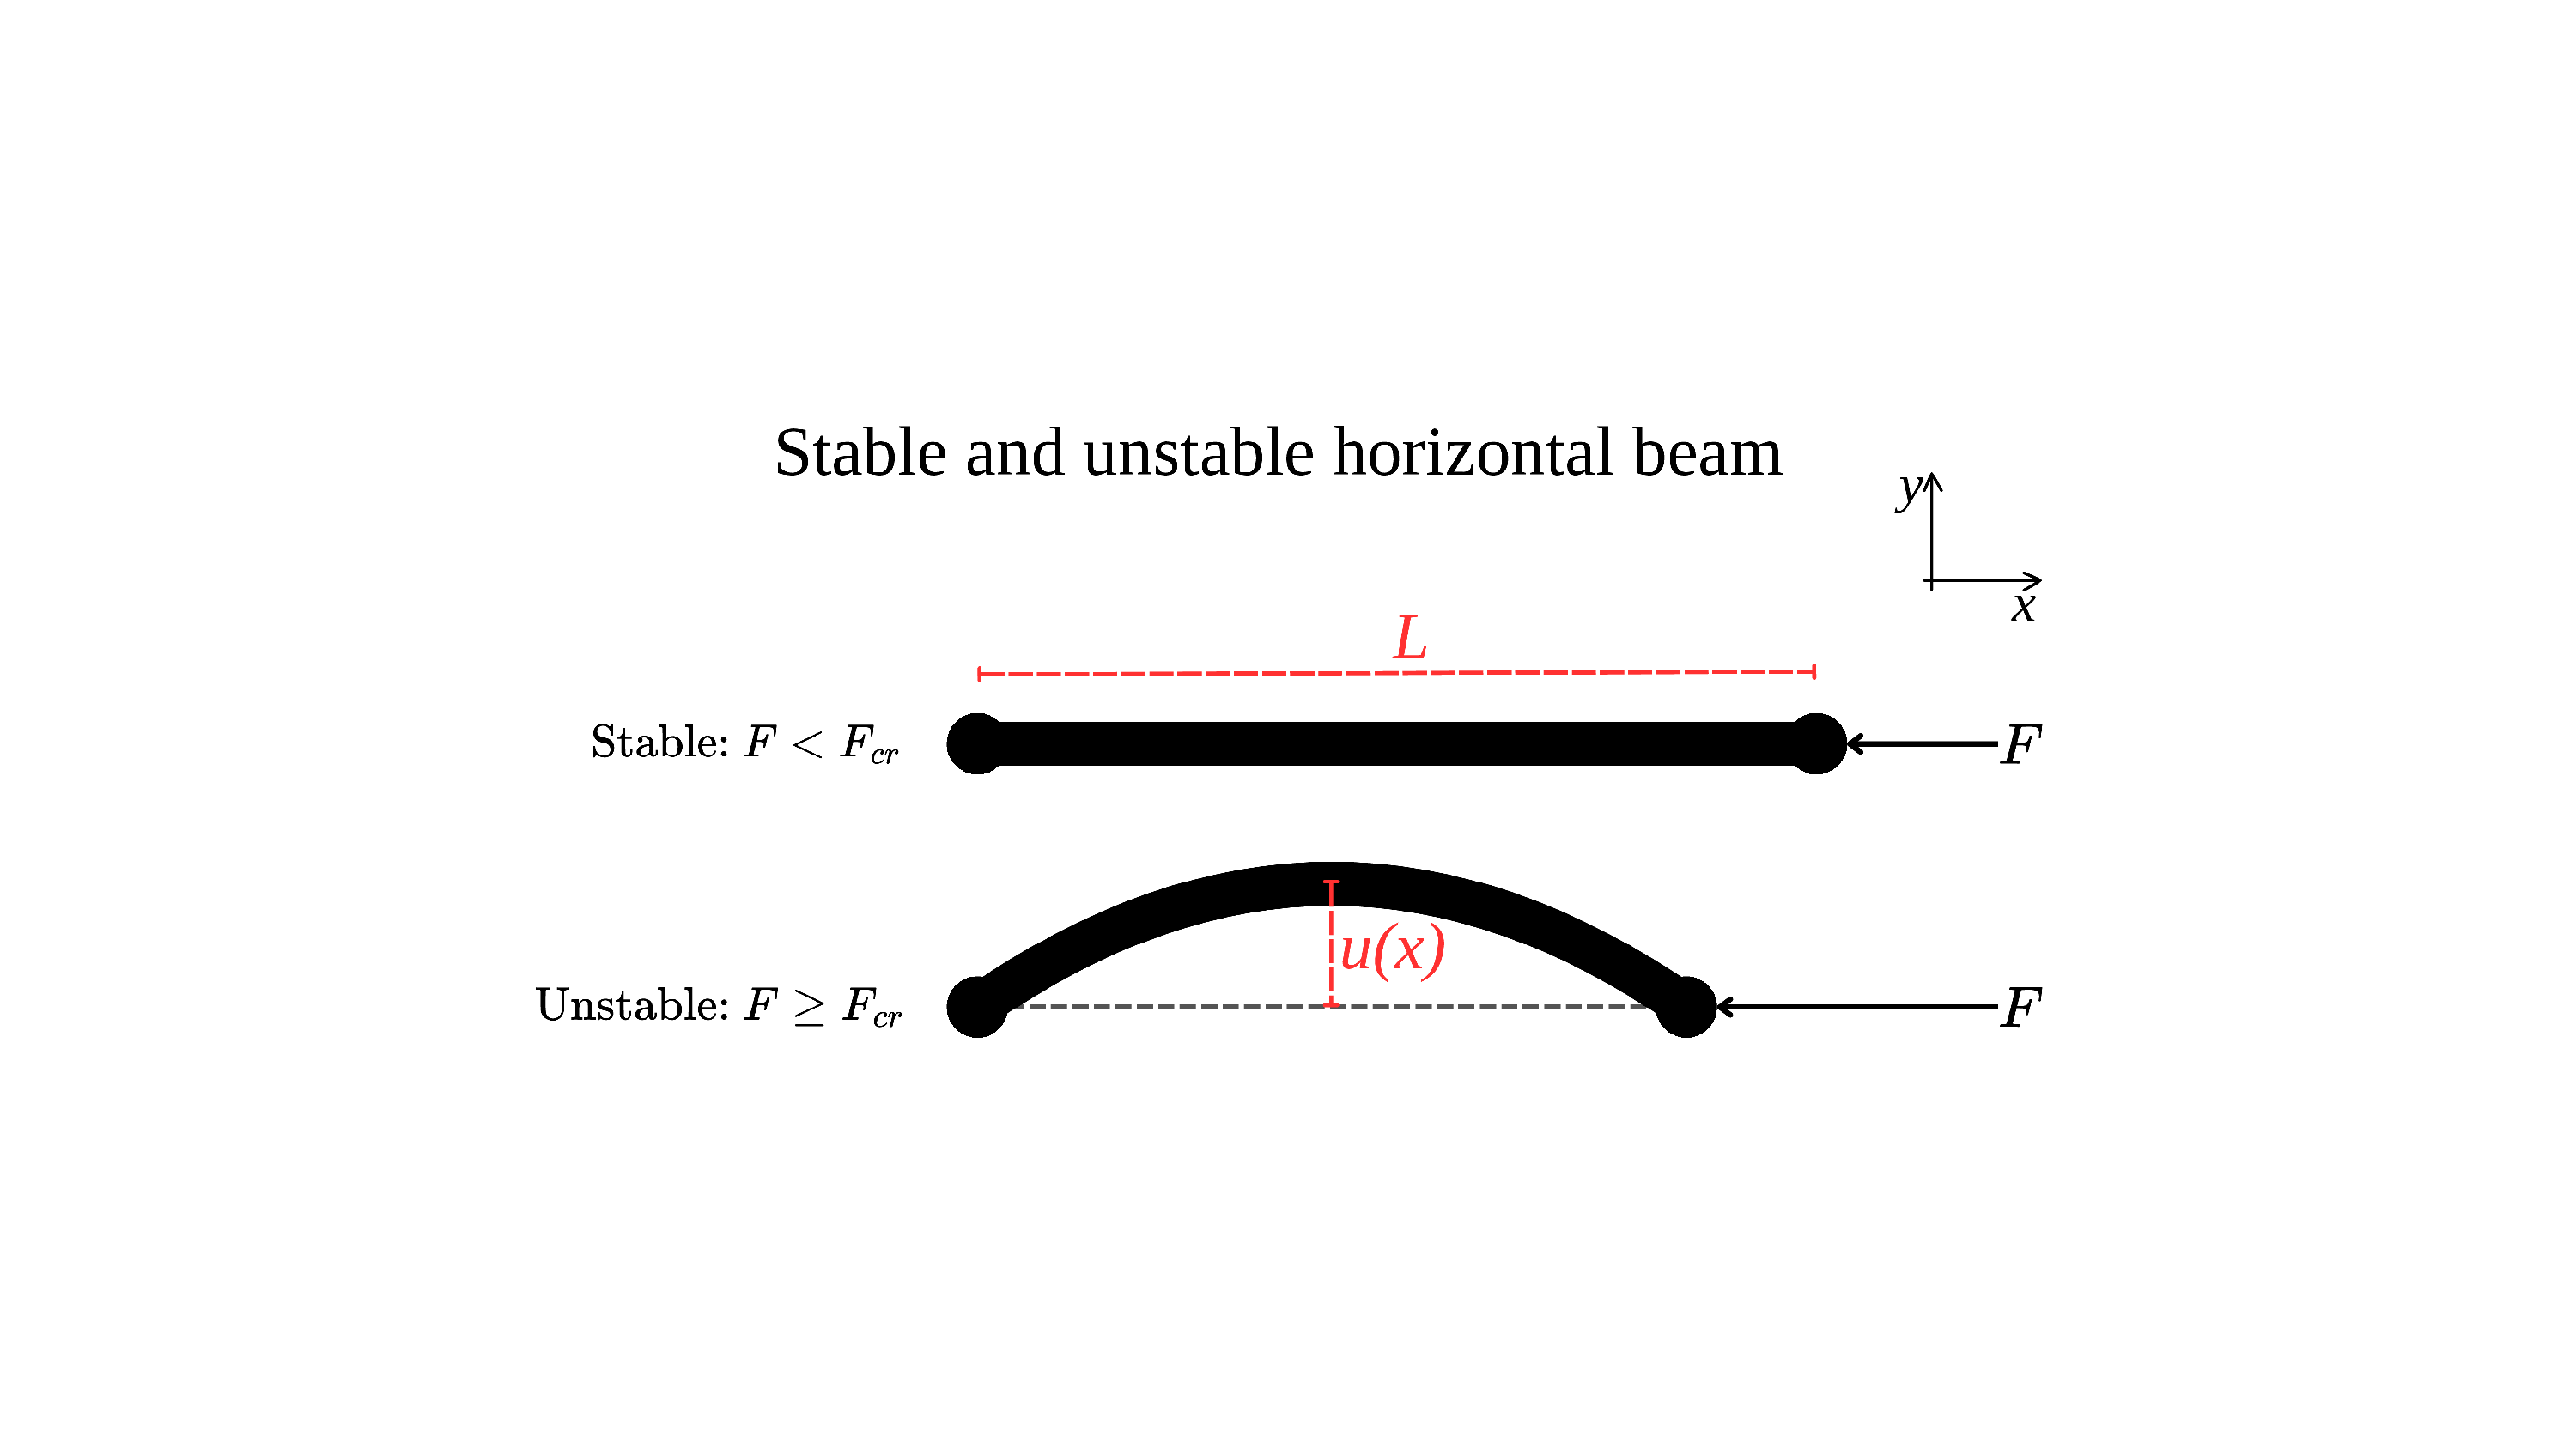
\includegraphics[width=.9\textwidth]{Project 2/Figures/horizontal_beam.pdf}
    \caption{The Beam under stable and unstable conditions. When the force $F$ at $x=L$ exceeds the critical force of the beam $F_{cr}$ it becomes unstable and buckles.}
    \label{fig:beam_illustration}
\end{figure}

To ease the process of solving equation \eqref{eq:1d_buckling_beam} we can performe a scaling of the equation by using the change of variables defined by $\hat x (x) := \hat x = \frac{x}{L}$. Under $\hat x$ the vertical displacement becomes $u_x(x) = u_{\hat x}(\hat x(x)):=u(\hat x)$. This variable change yields

\begin{equation*}
\eqref{eq:1d_buckling_beam}\quad \stackrel{\hat x = x/L}{\longrightarrow} \quad
    \gamma \frac{d^{2} u(\hat x)}{d (\hat x L)^{2}} = - F u(\hat x) \quad, 
\end{equation*}

which is easally rewritten to 
\begin{equation}\label{eq:1d_buckling_beam_scaled}
    \frac{d^{2} u(\hat x)}{d \hat x^{2}} = - \lambda u(\hat{x})  \quad ,
\end{equation}

where we defined $\lambda := \frac{FL^{2}}{\gamma}$. 


\end{document}
